\subsection{Физическая реализация маячка}

В плане физической реализации Beacon-маячки – это обычные Bluetooth 4.0 LE (Low Energy) устройства, таким образом, их роль может с успехом выполнять любое устройство, оснащённое BLE-чипом - например, cмартфоны на базе Android, а также iPhone, iPad, обычные ноутбуки, Raspberry Pi с usb bluetooth-донглом (электронным ключом) и т.д., на которое установлено специальное приложение, реализующее функции Beacon-маячка \cite{web:HabrBig}.

\begin{figure}[h]
    \centering
    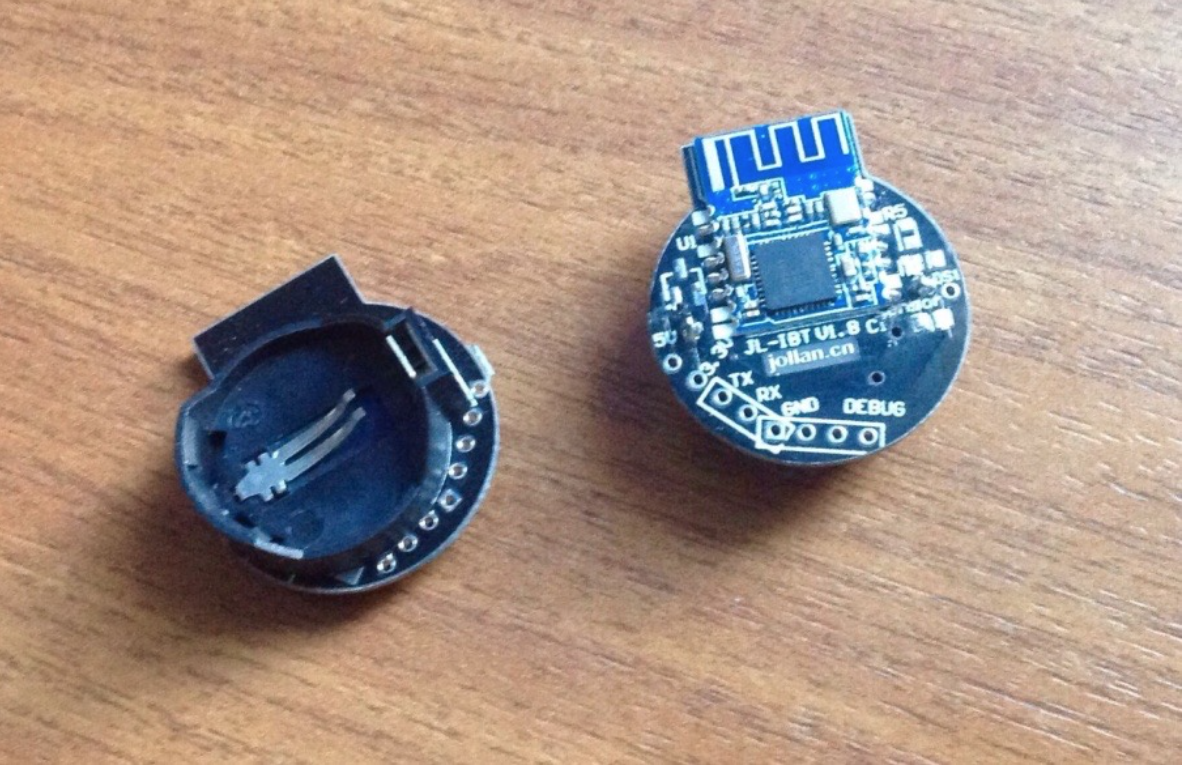
\includegraphics[scale=0.4]{img/beacons.png}
    \caption{Маячки, использованные в работе}
\end{figure}

Типичный маячок, показанный на рисунке выше, имеет довольно компактные размеры, и способен проработать всего лишь от одной батарейки до двух лет. Схемотехнически состоит из батарейки и Soc (System-On-Chip) Texas Instruments CC2540/2541 (также применяется Nordic nRF51822), представляющий собой 8051 микроконтроллер, в который загружается прошивка для реализации функции маячка и периферийный модуль Bluetooth LE. Дальность действия маячка в среднем 10 метров (варьируется от 15-20см до 25-40м в зависимости от модели и настроек). Периодичность выдачи данных - 200мс, но это, опять же, настраивается: можно настроить и на более частую периодичность, и на более редкую. В рассматриваемой работе маячки были настроены на периодичность в 1с. Срок службы от одной батарейки в зависимости от модели - от чуть менее одного года до трёх лет (в среднем 2 года). Цена одного маячка составляет порядка 15-20 долларов. Маячок является простым устройством, который только выдаёт всем подряд в эфир свои данные (в advertising-режиме), используя Bluetooth-профиль GATT (при этом к нему даже не нужно выполнять подключение), тем не менее, производители, как правило, закладывают возможность подключения к маячку с целью его удалённого конфигурирования (редактирование данных, выдаваемых в эфир, периодичность выдачи данных и мощность излучения), а так же решения вопросов безопасности.